\documentclass[a4paper, 12pt, oneside]{book}
\usepackage{hyperref}
\usepackage{listings,xcolor}
\usepackage[italian]{babel}
\usepackage{graphicx}
\usepackage{float}
\graphicspath{ {immagini/} }
\pagestyle{plain}
\begin{document}
\lstset{
    string=[s]{"}{"},
    stringstyle=\color{blue},
    comment=[l]{:},
    commentstyle=\color{red},
    breaklines=true,
}
\lstdefinelanguage{JavaScript}{
  keywords={typeof, new, true, false, catch, function, return, null, catch, switch, var, if, in, while, do, else, case, break},
  keywordstyle=\color{blue}\bfseries,
  ndkeywords={class, export, boolean, throw, implements, import, this},
  ndkeywordstyle=\color{darkgray}\bfseries,
  identifierstyle=\color{black},
  sensitive=false,
  comment=[l]{//},
  morecomment=[s]{/*}{*/},
  commentstyle=\color{purple},
  stringstyle=\color{red},
  morestring=[b]',
  morestring=[b]"
}
\setcounter{page}{1}
\pagenumbering{arabic}
%%Frontespizio
\begin{titlepage}
\begin{center}

\includegraphics[width=0.6\textwidth, height=0.15\textheight]{logo}
\\[1\baselineskip]
\Large Universit\'a del Piemonte Orientale
\\[2\baselineskip]
\Large Dipartimento di Scienze e Innovazione Teconologica
\\[1\baselineskip]
\textbf{\Large Corso di Studi in Informatica}
\\[2\baselineskip]
\normalsize Relazione per la prova finale
\\[1\baselineskip]

{\LARGE \bfseries Estensione di software di domotica\par con applicazioni per\par interazione\par uomo-macchina e\\ un'interfaccia di configurazione}\\[1cm]
\vspace{1cm}
\begin{minipage}[t]{0.4\textwidth}
\flushleft
{\bf Tutore interno:}\\
Prof. Marco Guazzone\\
\end{minipage}
\begin{minipage}[t]{0.4\textwidth}
\flushright
{\bf Candidato:}\\
Riccardo Berto\\
\end{minipage}
\vfill
\vspace{1cm}
\textbf{\large Anno Accademico 2016/17}
\vfill
\end{center}
\end{titlepage}

\newpage
%%Indice
\input{indice/indice}
\newpage
%%Capitoli
\input{capitoli/Introduzione}
\newpage
\chapter{Scopi e Problemi Affrontati}

\section{Applicazioni del MagicMirror}
Il Magic Mirror \`e un software che implementa api, le quali permettono
l'integrazione di applicazioni sviluppate da terzi e forniscono strumenti per la comunicazione, gestione
ed organizzazione tra di esse.
Lo scopo nello sviluppo delle applicazioni, durante lo stage, \`e stato
di creare programmi che permettessero l'interazione tra il software principale
e l'essere umano. Nello specifico si \`e voluto implementare la possibilit\`a, da parte di un utente,
di controllare le applicazioni attive sul Magic Mirror tramite l'impartizione di comandi vocali
o movimenti delle dita su una scheda touchpad.
In questa parte si \`e dovuto affrontare il problema di far comunicare
i diversi dispositivi hardware con il calcolatore principale, e di programmare
le applicazioni con linguaggi diversi, a seconda della compatibilit\`a di un linguaggio
e delle librerie a disposizione di una determinata periferica.
\\[2\baselineskip]
\section{Interfaccia di controllo del MagicMirror}
Nella seconda parte dello stage si \`e svolta la progettazione di un'interfaccia Web di configurazione remota
il cui scopo \`e di permettere ad un utente autenticato di gestire
le configurazioni delle applicazioni implementate nel software da una pagina web,
senza dover accedere fisicamente alla macchina.
Quest'ultima permette anche di disattivare (o attivare) le applicazioni presenti nel Magic Mirror,
la cui procedura, prima, richiedeva di aggiungere manualmente un pezzo di codice nella
configurazione del software princiapale.
Nello sviluppo dell'interfaccia si \`e affrontato il problema di dover modificare
il documento di configurazione del software principale senza eliminarne parti essenziali
o modificarlo in un formato sbagliato.
Lo scambio dei messaggi tra il Magic Mirror e la pagina web avviene in formato JSON, lo stesso formato
usato per il suo file di configurazione e delle sue applicazioni.\\
Un altro problema riscontrato in questa parte è stata la difficoltà dell'utilizzo di Javascript
perchè \`e un linguaggio asincrono, ovvero alcune funzioni venivano eseguite senza attendere
il risulato della precedente. Il linguaggio, per poter sincronizzare la funzioni, mette a disposizione
le callback: funzioni passate come parametro alla funzione principale che a loro volta avevano come paramentro il risultato,
in modo da poter eseguire le operazioni solo dopo che la funzione chiamante avesse prodotto l'output.
Il problema di questo approccio \`e stato il fenomeno "Callback Hell", ovvero Callback che chiamano a loro volta
altre Callback creando funzioni annidate pi\`u volte, come mostrato in figura \ref{fig:hell}.
\\[2\baselineskip]
\begin{figure}[h]
    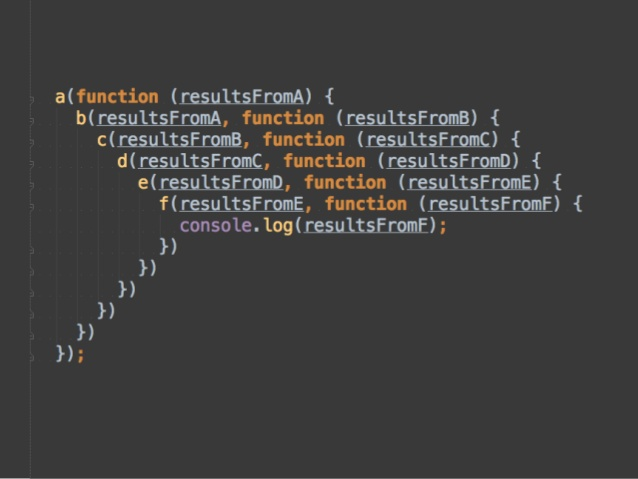
\includegraphics[width=1\textwidth, height=0.4\textheight]{callbackhell}
    \caption{Esempio di Callback Hell}
    \label{fig:hell}
\end{figure}

\newpage
\chapter{Tecnologie Implicate}
In questo capitolo verranno discusse le teconologie che sono state studiate ed utilizzate durante le attività di stage.
In particolare il capitolo è diviso tra teconologie hardware e tecnologie software.

\section{Prefazione}
Lo sviluppo del progetto \`e stato svolto nell'ambiente Raspbian\cite{Raspbian}
una distribuzione Debian\cite{Debian} che gira sul dispositivo RasperryPi\cite{Raspberry}.
Inoltre sono state adottate diverse tecnologie nel campo del riconoscimento vocale e di
immagini (OpenCV \cite{OpenCV-website} e Google Speech API \cite{GoogleSTT-website}),
nello sviluppo di applicazioni web (Electron \cite{Electron-website}, NodeJS \cite{NodeJS-website},
Express \cite{Express-website}, Mustache \cite{Mustache}), della gestione dati (MySQL \cite{MySQL}).
Inoltre sono stati adottati diversi linguaggi di programmazione (JavaScript \cite{JavaScript}, Python \cite{Python})
e piattaforme per la gestione distribuita di progetti softwave (GitLab \cite{git-website}).

\section{Hardware}
\subsection{RasperryPi}
RaspberryPi \`e un calcolatore elettronico, montato su una singola scheda elettronica,
caratterizzato dal basso costo, dal consumo energetico ridotto e, per le sue
dimensioni ridotte, dalla facile portabilit\`a.
Rilasciato per la prima volta nel 2012 \`e diventato un prodotto utilizzato per una moltitudine
di progetti sia aziendali che casalinghi.
Il modello usato durante lo stage \`e RaspberryPi 3 model B e monta:
\begin{itemize}
\item CPU con architettura ARM (Advanced RISC Machine)
\item 1 porta HDMI
\item 1 porta LAN
\item 1 uscita Aux
\item 4 porte USB
\item 40 pin General Purpose Input/Output(GPIO)
\item 1 scheda di rete wireless
\item Alimentazione microUSB 5V
\item un bus camera serial interface(CSI), ovvero una porta per telecamere con Flexible flat cable(FFC)
\item ingresso per microSD
\end{itemize}
Il sistema operativo per Raspberry deve essere installato su una microSD opportunamente formattata
e configurata con un Master Boot Record (MBR).

\subsection{Periferiche}
Nella creazione delle applicazioni per il Magic Mirror sono state usate diverse periferiche, tra cui un microfono
USB, per catturare la voce in input e un componente Skydriver Touch Board (94mm x 122mm) di Piromoni collegabile tramite
i 40 pin GPIO del calcolatore principale, per catturare input fisici tramite il movimento delle dita sulla Touch Board.

\section{Software}
\subsection{Raspbian}
Raspbian \`e una distribuzione del sistema operativo Linux derivata da Debian, completamente libera,
ottimizzata per Raspberry.
Fu sviluppata da Mike Thompson e Peter Green come progetto non affiliato alla compagnia RaspberryPi
Fundation, per tenere in considerazione la limitata capacità di calcolo dei processori ARM.
La prima versione venne rilasciata nel 2012.

\subsection{Electron}\label{cap:Electron}
Electron \`e un framework open source rilasciato per la prima volta nel 2013, ma la prima versione
stabile \`e uscita durante giugno 2017. \`E disponibile per i sistemi operativi Windows, MacOS e Linux ed \`e scritto
in C++ e Javascript. Il framework permette la creazione di applicazioni multipiattaforma
utilizzando teconologie gi\`a esistenti per lo sviluppo
del lato client e del lato server (Javascript, NodeJS, V8 \cite{V8}).
All'avvio di Electron viene inizializzata una pagina con Chromium \cite{Chromium}(un web browser installato insieme all'applicazione)
nel quale viene mostrata una pagina web, e un server in NodeJS.
Un'applicazione sviluppata con Electorn ha bisongo di 3 componenti principali:
\begin{itemize}
\item Il package.json, un file JSON, che deve contenere almeno il nome dell'applicazione,
la versione dell'applicazione creata, la descrizione di quest'ultima e il
 nome del file principale dell'applicazione (necessaria per l'avvio), come mostrato nella
 seguente immagine:
\begin{lstlisting}
{
  "name": "magicmirror",
  "version": "2.1.1",
  "description": "The open source smart platform",
  "main": "js/electron.js"
}
\end{lstlisting}
Name è il campo che assegna il nome dell'applicazione, version è il cmapo che assegna la versione
dell'applicazione, description è una stringa che descrive il programma, main è il cmapo che punta al file
Javascript eseguibile
\item Un file HTML che contiene il template della pagina generata dall'applicazione
\item Un file JavaScript che contiene il codice di esecuzione dell'applicazione come ad esempio la
creazione di una finestra o la visualizzazione di una pagina.
\end{itemize}

\subsection{OpenCV}
OpenCV (Open Source Computer Vision Library) \`e una libreria software sviluppata intorno al 2000
utilizzata nell'ambito della visione artificiale per l'acquisizione e il riconoscimento di immagini
da parte di una macchina per mezzo di input digitali, ottenuti tramite telecamera o fotocamera.\\
La libreria \`e disponibile per i linguaggi C++(linguaggio in cui \`e scritta), C, Python e Java e
per diversi sistemi operativi, compresi quelli specifici per i dispositivi mobili.\\
OpenCV prende in input un'immagine o uno stream (come un video o una serie di immagini) e, l'utilizzo di
specifici algoritmi di Machine Learning per individuare e riconoscere oggetti specifici.

\subsection{Google Speech API}
Negli ultimi anni Google ha ampliato sempre di pi\`u il suo catalogo per quanto riguarda
i servizi cloud e web API.
Tra questi si pu\`o individuare anche Google Speech API, il quale \`e un
servizio che, ricevendo in input un file o uno stream audio, ottenuto per mezzo di un'acquisizione
da un dispositivo di audio input, traduce il parlato in testo scritto tramite algoritmi avanzati
di riconoscimento della voce.\\
L'API supporta oltre 110 lingue e si possono usare su diverse piattaforme dato che
le librerie sono disponibili nei linguaggi C\#, GO, Java, Node.JS, PhP, Python e Ruby.
Inoltre Google Speech To Text dispone di alcune varianti:
\begin{itemize}
\item Una con interfaccia REpresentational State Transfer(REST), che comunica per mezzo di URI
\item Una con gRPC, un sistema di chiamata di procedura remota
\end{itemize}

\iffalse
\section{Model-View-Design}
Il Model-View-Design (MVC) \`e un pattern architetturale che suddivide lo sviluppo di un'applicazione web in 3 parti:
\begin{itemize}
\item Model(Modello), sono oggetti che rappresentano lo stato dell'applicazione e operazioni logiche da eseguire sul primo. Di solito
lo stato del modello viene estratto, manipolato per mezzo di operazioni e salvato da un database con cui comunicano,
oppure passato al controller.
\item Controller, \`e un'interfaccia che comunica tra il Model, la View e l'Utente. Il suo compito \`e di gestire le richieste dell'utente,
il quale comunica tramite input ed interazioni, utilizzando il modello che rientra nel dominio
dei dati inerente alla richiesta e selezionando una View per il rendering dell'interfaccia utente.
\item View(Visualizzazione), ha il compito di far visualizzare all'utente i dati estratti tramite un'interfaccia grafica, che viene creata
partendo da un modello HTML.\\[2\baselineskip]
\end{itemize}
\begin{figure}[H]
    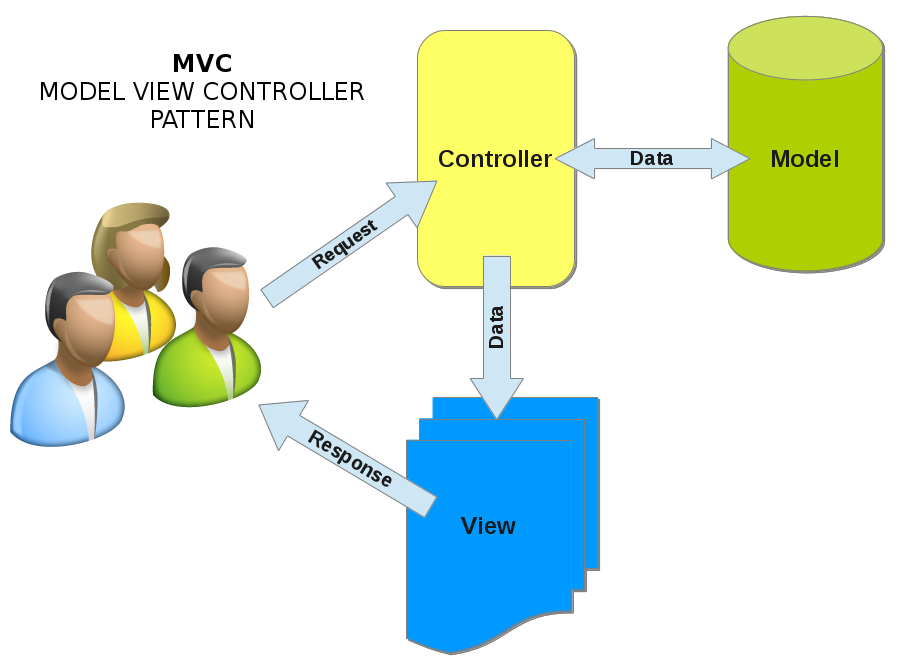
\includegraphics[width=0.9\textwidth]{mvc}
    \caption{MVC Pattern}
\end{figure}
\fi

\subsection{Node.JS}
Node.JS era già implementato con Electron, ed è stato usato per la creazione del server
per la gestione dell'interfaccia web per il MM.
Node.JS \`e una piattaforma open source che permette l'esecuzione del linguaggio Javascript
anche per il lato server, ovvero
la parte del sistema che contiene applicazioni e programmi  scritti, in questo caso, in Javascript
ed eseguiti sfruttando il motore JavaScript V8 sviluppato da Google.
Il lato server è una parte del sistema che l'utente, di solito, non interagisce direttamente
e che ne permette l'effettivo funzionamento e, nel caso, la manipolazione e l'elaborazione
dei dati.\\
Node.JS esegue delle operazioni al verificarsi di uno specifico evento, che pu\`o essere un accesso ad una porta
del server o la richiesta di una pagina.
Per gestire i pacchetti di questo framework viene utilizzato NPM\cite{NPM}, uno strumento che permette
di scaricare ed installare librerie private o pubbliche salvate su un database.
\\[1\baselineskip]

\subsection{Express}\label{cap:express}
Express \`e un framework per Node.JS che permette di creare applicazioni Web e API in JavaScript, offrendo strumenti e pacchetti
che implementano più facilmente tutti i servizi (e anche di più) offerti da Node.JS.
Il software viene usato per creare e gestire il backend di un server, che \`e composto di 3 entit\`a importanti:
\begin{itemize}
\item il Controller, che definisce le funzioni associate ad un determinato modello.
\item il Routing, utilizzato per determinare come il server debba rispondere ad un determinato metodo di richiesta,
ricevuta sottoforma di URI, inoltrando la richiesta alla funzione del controller del modello a cui fa rifermento.
\item i Modelli, creati per ogni entit\`a-oggetto che esiste all'interno del server, ad ognuno dei quali viene associato
un controller. Inoltre, tramite i modelli si accede al databse per estrarre i dati e spedirli al controller per
la manipolazione, ricevendoli successivamente modificati e salvandoli, se necessario.
\\[2\baselineskip]
\end{itemize}

\subsection{Mustache}
Mustache è un motore di template disponibile per molti linguaggi tra cui Javascript.
\`E stato usato come motore di template per l'interfaccia web di configurazione
del MagicMirror.
Mustache è un sistema logic-less perchè è privo di istruzioni per il controllo del flusso
(come ad esempio l'if e l'else), quindi tutti i controllli di questo tipo vengono fatti
attraverso programmazione data-driven.
Il nome di questo motore è dovuto all'utilizzo delle parentesi graffe, usate spesso
all'intero della sua sintassi, che, se viste da una certa angolatura, assomigliano
a un paio di baffi.

\subsection{MySQL}
MySQL è stato usato durante lo stage per l'archiviazione di utenti con i permessi accedere all'interfaccia web del MM.
MySQL è uno tra i più famosi database open source sviluppato da Oracle, più precisamente
è sistema per la gestione di basi di dati basato sul modello relazionale.
MySQL è composto da una semplice riga di comando e un server web, ma sono implementati anche programmi
per l'amministrazione del database (come ad esempio il famoso phpMyAdmin).
La prima versione fu rilasciata nel maggio del 1995 Sviluppato da Oracle e di proprietà di MySQL AB,
distribuito sia con licenza commerciale sia con licenza libera.

\subsection{JavaScript}
Javascript \`e un linguaggio di programmazione ad alto livello orientato agli oggetti e ad eventi, che \`e supportato da tutti i browser
per lo scripting delle pagine web, e che supporta la programmazione procedurale.
Inizialmente usato per il lato client ha subito un'evoluzione che lo ha portato ad essere utilizzato per lo sviluppo di backend e web app.
\\[2\baselineskip]
ECMAJavascript(ES) \`e lo standard di Javascript che negli ultimi anni ha sviluppato ed evoluto il linguaggio in diverse versioni.
In tutte il problema pi\`u trattato \`e il fatto che Javascript \`e orientato agli eventi,
ed alcune funzioni necessitano di Callback, che possono degenerare se non vengono
utilizzati buone pratiche di programmazione. Le callback sono necessarie perch\`e alcune chiamate di funzioni non vengono fatte direttamente, ma vengono
fatte attraverso messaggi, i quali vengono salvati in una coda di messaggi e vengono spediti sequenzialmente ad uno stack di chiamata dove
viene salvata la corrispondente funzione per l'esecuzione. Questo metodo rende il linguaggio asincorno perch\`e le funzioni e gli eventi
vengono eseguiti in successione senza attendere il termine della precedente.
\\[1\baselineskip]Le soluzioni adottate in ECMA Javascript 5 (ES5), la versione usata durante lo
stage, sono l'utilizzo delle Callback già discusse nella sezione 1.2 (label).
\\[1\baselineskip]
In ECMA Javascript 6 (ES6) sono state introdotte le Promises, ovvero al posto di far tornare una funzione Callback, ritorna una Promise(Promessa),
la quale garantisce che una variabile/oggetto avr\`a un ritorno, mettendo cosi la funzione in attesa fino al ricevimento del valore o di un errore.
Sono tutt'ora in via di sviluppo nuove versioni di Javascript.

\subsection{Python}\label{cap:python}
Questo linguaggio \`e stato particolarmente utile per l'interfacciamento con la telecamera e la Touch Board, essendo a disposizione librerie
apposite per gestirle.
Python \`e un linguaggio di programmazione open source, ad alto livello con semantica dinamica, orientato ad oggetti, usato
per sviluppo di applicazioni e scripting.\\[1\baselineskip]
Come molti altri linguaggi supporta pacchetti anche sviluppati da terzi, salvati in una repository pubblica,
attraverso un suo gestore di pacchetti Pip Installs Packages o Pip Installs Python (pip, acronimo ricorsivo).
\\[1\baselineskip]
Inoltre con Python \`e possibile creare ambienti isolati per l'utilizzo di pacchetti e moduli senza doverli installare all'interno del sistema.
Per poterlo fare \`e disponibile virtualenv, uno strumento Python che permette, appunto, di creare ambienti virtuali (virtual enviroments).
\\[2\baselineskip]

\subsection{GitLab}
GitLab \`e una piattaforma web che implementa le funzionalit\`a offerte dal software Git e altri
servizi tra i quali la possibilit\`a di creare wiki e un servizio di issue tracking, utile per tenere traccia
di eventuali richieste o problemi.
La comodità di questa piattaforma sta nel poter creare dei Commit, ovvero ad ogni modifica del codice si può
salvarne lo stato assegnadoli un'etichetta in locale, per poi spedire la versione al remoto del progetto.
In ogni momento si può tornare ad una versione vecchia tramite gli strumenti di reversering offerti dal servizio.

\newpage
\chapter{Struttra del Magic Mirror}

Il Magic Mirror \`e un progetto ideato e sviluppato da Michael Teeuw, successivamente esteso nelle sue funzionalit\`a da una moltitudine di utenti su GitHub.
Una prima versione \`e stata scritta completamente in Python, mentre, in seguito, \`e stata creata una seconda versione nella quale si \`e preferito l'utilizzo di Electron,
che ha comportato una variazione di linguaggio, a favore di Javascript. In questo modo \`e stato possibile implementare un'interfaccia esteticamente pi\`u gradevole
e api pi\`u intuitive.
\\[2\baselineskip]

\section{Perch\`e Magic Mirror?}
L'idea dell'autore \`e nata rifacendosi allo specchio magico dell'omonima fiaba
scritta dai fratelli Grimm, La Bella Addormentata.\\
Il software viene mostrato attraverso un
comune monitor, trasmettendo immagini poste su uno sfondo completamente nero. Applicando sopra
una semplice pellicola a specchio (la quale da un lato permette di specchiarsi e dall'altro di vedere
attraverso) si crea un effetto particolare per cui una persona riesce a specchiarsi
e allo stesso tempo riesce a vedere le scritte o le immagini trasmesse dal monitor.
\\[2\baselineskip]
\begin{figure}[H]
    
\includegraphics[width=1\textwidth, height=0.6\textheight]{magic_mirror}
    \caption{Magic Mirror by Michael Teeuw}
\end{figure}

\section{Avvio ed Escuzione}
Il Magic Mirror viene avviato tramite riga di comando di una shell: npm start, che va a ad eseguire
il codice di un file javascript indicato dal file package.json.
Il primo contiene il codice di Electron, che si occupa della creazione di una nuova finestra, che rappresenta l'interfaccia contenente il browser
contetente i Document Object Model(DOM), e il codice dell'applicazione, ovvero il corpo principale dello specchio.
Quest'ultima carica tutte le strutture dello specchio:
\begin{itemize}
\item le api per le applicazioni, che sono le interfacce usate per leggere e caricare le applicazioni inserite nel Magic Mirror.
\item le api per i Node Helper, interfacce per i Node Helper di una applicazione, sono strutture opzionali usate per collegamenti
esterni al Magic Mirror(per esempio con api di un servizio cloud). Ogni applicazione ha il proprio Node Helper con cui pu\`o comunicare tramite messaggi in modo
simile a come comunicano le applicazioni tra di loro.
\item un "Socket", entit\`a principale che definisce le funzioni e le metodologie per lo scambio dei messaggi tra le applicazioni e i rispettivi Node Helper.
\item un Logger, implementato per tenere i log dell'applicazione e degli evenutali errori. Usato pricipalemnte per il debugging.
\item un file Config, un file di configurazione dello specchio, nel quale sono segnate il nome e le coordinate per la posizione all'inteno della pagina\\[2\baselineskip]
\end{itemize}
Inoltre viene inzializzato un server il quale ha il compito di trasmettere la pagina renderizzata sulla base
degli output delle varie applicazioni al browser avviato inizialmente.

\subsection{Il file di Configurazione}
Come già menzionato il Magic Mirror carica un file di configurazione, il quale ha al suo inteno:
\begin{itemize}
\item la porta del server
\item una whitelist ovvero un ip oppure un range di ip che possono collegarsi allo specchio
\item la lingua principale del sistema
\item il formato del timer (12h o 24h)
\item unità di misura usata (per esmepio metrica)
\item una lista di applicazioni (in formato JSON) da caricare con la relativa posizione nella pagina. Necessarimaente per ogni applicazione deve comparire il
nome e la posizione, opzionalmente si possono inserire un campo header e un campo config specifico per l'applicazione:
\begin{lstlisting}
{
	"module": 'nome dell'applicazione',
	"position": 'la posizione dell'applicazione',
	"header": 'stampa sopra all'applicazione',
	"config": { opzioni varie in formato JSON }
}
\end{lstlisting}
\end{itemize}
La lingua, il formato del timer e l'unità di misura usata sono strumenti che possono essere utilizzati nella creazione di un'applicazione
(per esempio il display di un orologio).

\section{Specifiche delle applicazioni}
La modifica del file di configurazione, appena descritta, del Magic Mirror serve per notificare la presenza delle applicazioni a quest'ultimo,
ma perchè possano funzionare è necessario che si trovino in una specifica cartella e rispettino delle specifiche regole.
Per inserire il codice dell'applicazione all'interno dello specchio è necessario creare una cartella con uno nome identificativo dell'applicazione
nella directory "Modules".
Dentro la cartella appena creata devono essere inseriti:
\begin{itemize}
\item 1 file Javascript(JS), il documento principale con lo stesso nome della cartella appena creata, contiene il codice il codice dell'applicaizone, il quale
conterrà ance il codice per la creazione dei DOM
\item 1 file Cascading Style Sheets(CSS), opzionale, per modificare l'esetica del DOM della relativa applicazione
\item 1 file node\_helper.js, opzionale, che è il Node Helper associato alla specifica applicazione
\item Altri file necessari all'applicazione (file.js)
\end{itemize}
Il file javascript principale viene caricato dal Magic Mirror, ed è composto dalla chiamata una funzione passando due parametri:
\begin{lstlisting}[language=JavaScript]
{
	Module.register("Nome del Modulo", { /* varie funzioni passate in formato json */});
}
\end{lstlisting}
Il primo parametro è una stringa che rappresenta il nome del modulo, il quale deve essere necessariamente uguale a quello della cartella e del file Javascript,
mentre il secondo è un file JSON contenente una lista di parametri di cui alcuni definiti.

\section{Messaggistica del MM}
adasd

\newpage
\chapter{Applicazioni per il MM}\label{capitolo4}
In questo capitolo vengono spiegati i requisiti dei moduli sviluppati durante lo stage e la loro implementazione.
In particolare verranno esposte le dipendenze per il modulo dei comandi vocali (sezione \ref{cap:sox}), le metodologie
per accedere ai sevizi di Google (sezione \ref{cap:google}), come avviene la comunicazione tra l'API e il programma (sezione \ref{cap:api})
e l'implementazione del modulo con Touch Board (sezione \ref{cap:touch}).

\section{Modulo per comandi vocali}\label{cap:voce}
La prima applicazione implementata, come \`e stato accennato nell'introduzione del capitolo \ref{capitolo4}, \`e
stata il controllo del MagicMirror tramite comandi vocali.
Nello specifico l'applicazione deve, tramite delle specifiche frasi,
gestire le altre applicazioni presenti nel MagicMirror, sfruttando funzioni offerte dallo stesso.\\
Nella figura \ref{fig:modulovocale} \`e rappresentata la struttura e il funzionamento del modulo.
Il microfono cattura l'audio, che viene elaborato, all'interno del NodeHelper, dal software Sound eXchange (\textit{SoX}), un software per l'elaborazione e la manipolazione
dell'audio. Successivamente, l'audio così elaborato, viene
passato all'API Speech To Text, la quale lo inoltra al Servizio Google Speech e si mette in attesa di una risposta.
Al ritorno di questa, viene passata al modulo che ha il compito di validare il comando e di inoltrarlo ai moduli, se
corretto.
Per poter utilizzare l'API \`e necessario installare il software SoX e fornire un'autenticazione per i servizi Google.

\begin{figure}[H]
    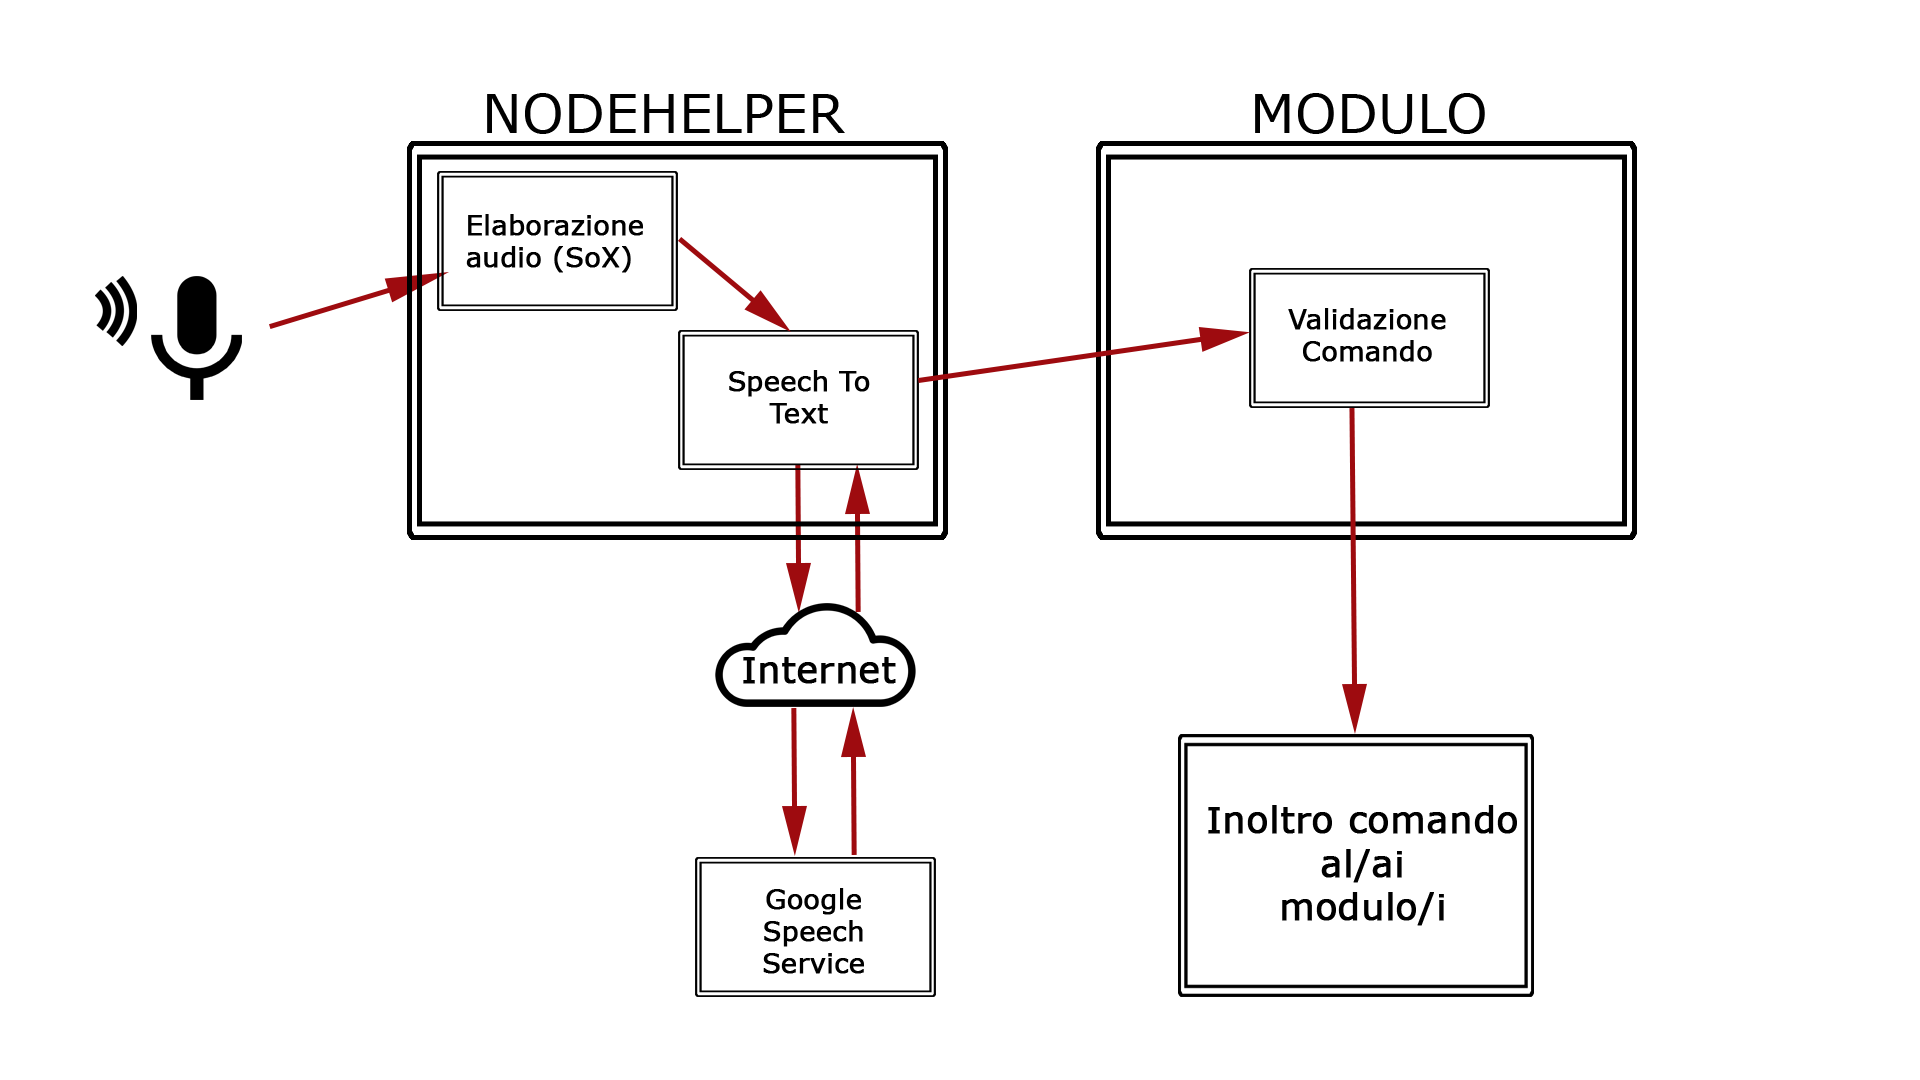
\includegraphics[width=1\textwidth, height=0.4\textheight]{modulovocale}
    \caption{Struttura del modulo per comandi vocali}
    \label{fig:modulovocale}
\end{figure}

\subsection{Comunicazione con l'API}\label{cap:api}
Il NodeHelper dell'applicazione si occupa di gestire lo streaming con l'API e
di mandare i risultati (o gli errori) all'applicazione tramite le funzioni messe
a disposizione dal MagicMirror, esposte nella sezione \ref{cap:MMmess}.
Il seguente codice viene usato per creare un canale streaming con l'API:
\begin{lstlisting}[language=Javascript, caption={Codice per l'inoltro dell'audio al Servizio Google}, captionpos=b]
      const recognizeStream = speech.streamingRecognize(request)
        .on('error', sendSocketNotification("error"))
        .on('data', (data) =>
          if(Transcription: ${data.results[0].alternatives[0].transcript})
            sendSocketNotification('limit_reached')
          else
            sendSocketNotification('response', data.results[0])
\end{lstlisting}
\emph{speech.streamingRecognize(request)}, richiama la funzione dell'API per aprire una connessione, dove \emph{request} \`e
il flusso audio.
La funzione si mette successivamente in attesa di una risposta dall'API la quale pu\`o essere di due tipi:
\begin{itemize}
\item errore, nel caso ci sia stato un errore di connessione. In questo caso viene mandato al modulo un messaggio di errore
\item dati di risposta, nel caso di risposta senza errori, ma che pu\`o essere divisa uteriormente in altre due risposte. La prima sia ha nel caso in cui
viene raggiunto il limite di parole tradotte (Google mette a disposizione un limite giornaliero per chi vuole usufruirne gratuitamente). In questo caso
il modulo lo notificherebbe a video con un messaggio di errore. La seconda risposta contiene una stringa con la frase tradotta,
che il modulo validerebbe come comando,
e, in caso di risposta positiva, la inoltrerebbe ai moduli.\\[1\baselineskip]
\end{itemize}
Per passare il flusso audio alla funzione appena descritta bisogna creare una \emph{pipe}, ovvero uno strumento
per permettere a due processi di comunicare.
Nel seguente codice:
\begin{lstlisting}[language=Javascript]
      // Start recording and send the microphone input to the Speech API
      record
        .start({
          sampleRateHertz: 1600,
          threshold: 0,
          verbose: false,
          recordProgram: 'sox',
          silence: '20.0'
        })
        .on('error', sendSocketNotification('error'))
        .pipe(recognizeStream);
\end{lstlisting}
\emph{record} \`e una funzione con ascolto di eventi che
imposta tramite il metodo \emph{.start} i settaggi dello streaming (per esempio la frequenza) e ne inizia la cattura.
L'evento \emph{.on('error')} serve per sollevare un'eccezione in caso di errore, che poi viene inoltrata al modulo.
L'evento \emph{.pipe(recognizeStream)} crea una pipe tra la funzione di registrazione e \emph{recognizeStream} descritta nel codice precedente,
passando il flusso audio direttamente alla funzione.

\subsection{Difficolt\`a incontrate}
\subsubsection{Sound eXchange (SoX)}\label{cap:sox}
Per permettere all'audio di venire correttamente elaborato
per lo streaming, \`e necessario utilizzare Sound eXchange (SoX), citato nella sezione \ref{cap:voce}.
Affinch\`e il microfono si colleghi correttamente al programma \`e necessario impostare correttamente
i valori delle varibili d'ambiente \textit{AUDIODEV} e \textit{AUDIODRIVER}.
La prima variabile corrisponde al dispositivo audio al quale il programma deve fare riferimento,
la seconda varibile al driver audio da utilizzare; di solito il predefinito \`e Advanced Linux Sound Architecture(ALSA).

\subsubsection{Autenticazione Google API}\label{cap:google}
Per poter usufruire delle API di Google \`e necessario fornire un'autenticazione a livello
di sistema.
Per poterlo fare bisogna ottenere delle credenziali di sicurezza per un account Google,
attivabili tramite Google Cloud Platform Console.
Le credenziali consistono in un username, l'email dell'account Google e una chiave di sicurezza unica,
 il tutto contenuto in un file JSON che pu\`o essere scaricato e salvato in locale.
Per poter permettere al sistema di utilizzare l'API occorre che il file JSON con le credenziali sia
raggiungibile all'interno del sistema e per rendere possibile ciò, bisogna creare una variabile d'ambiente con assegnato il percorso
dove si trova il file.

\section{Modulo con Touch Board}\label{cap:touch}
Nell'implementazione del modulo con la Touch Board \`e necessario aver installato nel sistema
il linguaggio di programmazione Python, descritto nella sezione \ref{cap:python}.\\
La Touch Board si presenta come una scheda con 40 porte I/O (le quali devono essere collegate alle
GPIO della scheda RaspberryPi) e con un sensore elettrico di prossimit\`a, come mostrato in figura \ref{fig:TouchBoard}, che permette di catturare i movimenti fino a
5 cm di distanza.
Le librerie Python, in dotazione con la scheda, offrono funzioni per catturare i diversi input trasmessi, come ad esempio
la direzione di spostamento del dito, oppure la cattura di un tocco sulla scheda.\\
La struttura del modulo, mostrata in figura \ref{fig:structtouch}, \`e composta da un'entit\`a che, al ricevimento di un input
sulla Touch Board, elabora e riconosce l'input ricevuto e lo inoltra al modulo.
Il comando viene validato e, in caso di risposta positiva, viene inoltrato agli altri moduli.
Per poter eseguire un programma Python sul MM \`e necessario usare la libreria Javascript \emph{Python-Shell}, la quale
permette di avviare una shell di Python in background e avviare, di conseguenza, i programmi.
La comunicazione tra programma Python e il NodeHelper avviene tramite messaggi in JSON. Quando la scheda riceve un input,
il programma Python comunica il risultato al NodeHelper che lo inoltra al modulo.

\begin{figure}[H]
    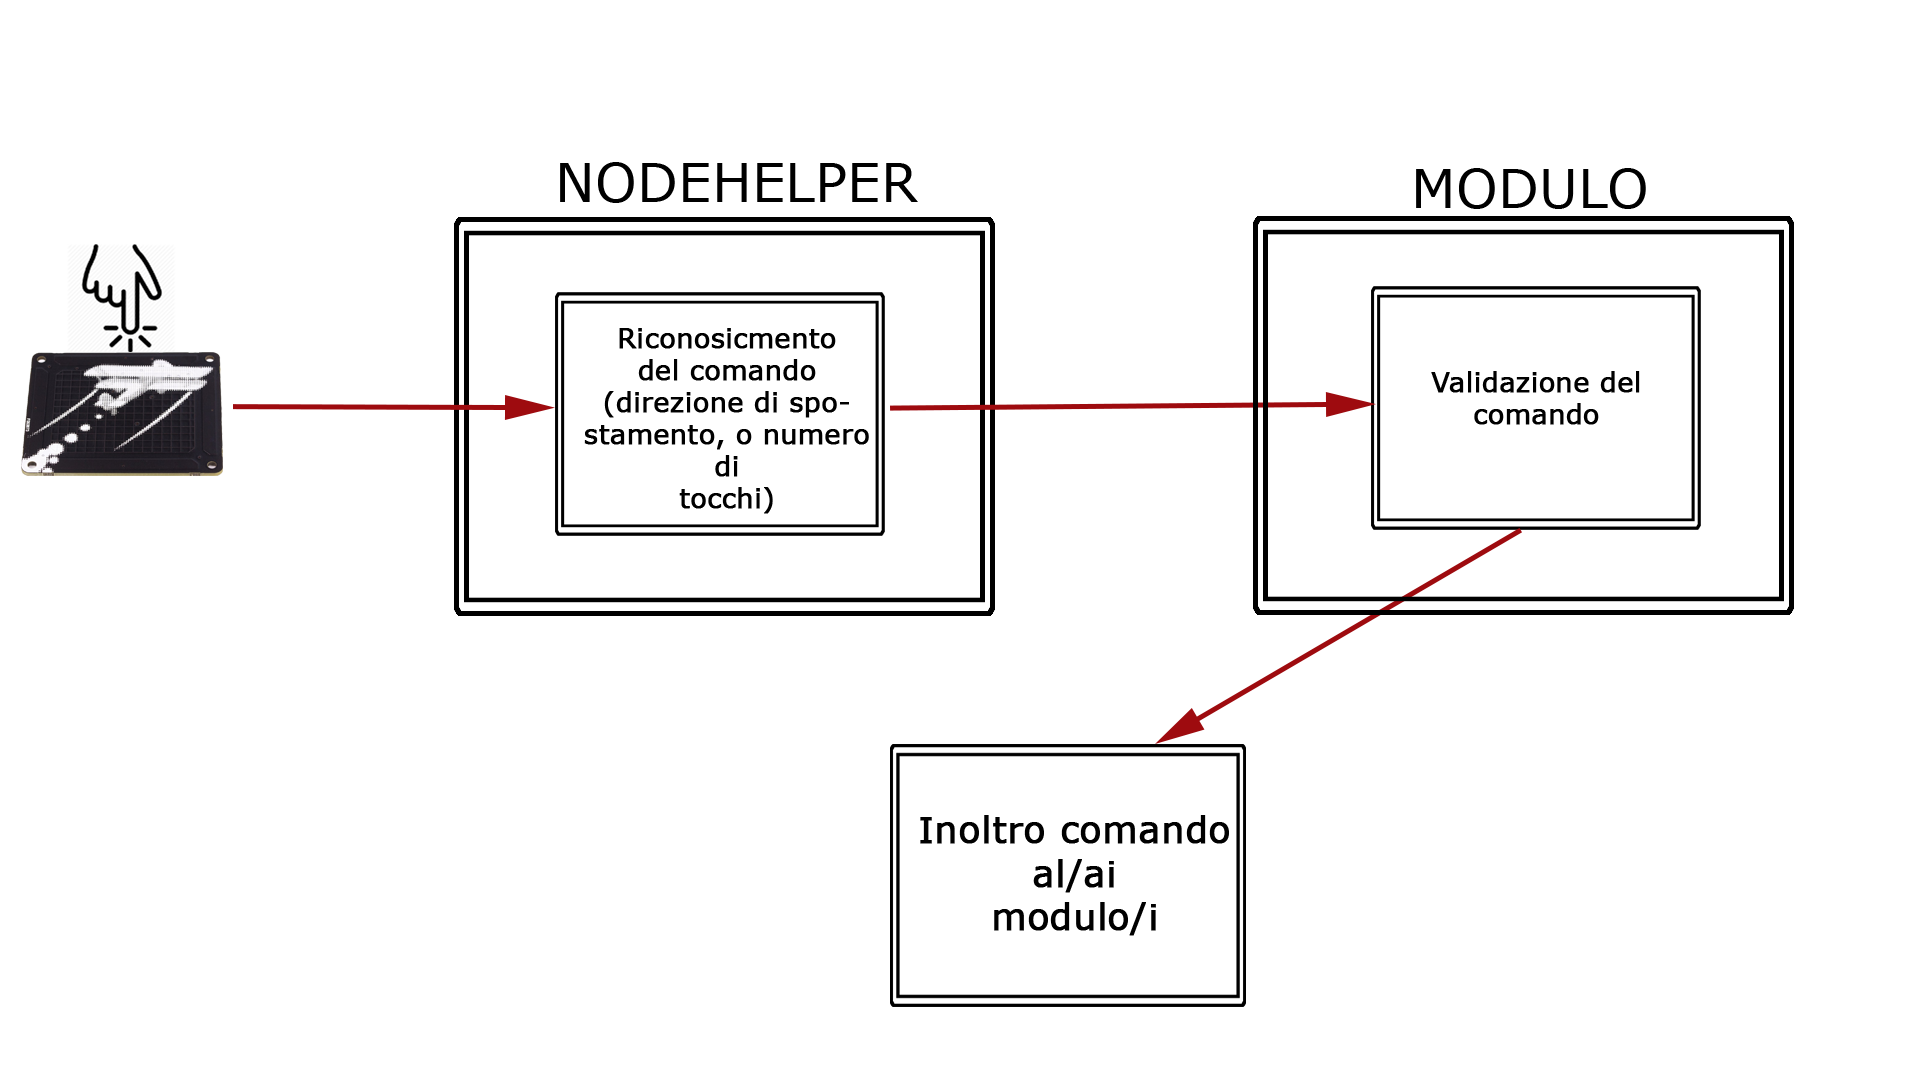
\includegraphics[width=1\textwidth, height=0.4\textheight]{touchstruct}
    \caption{Struttura del modulo con la Touch Board}
    \label{fig:structtouch}
\end{figure}

\begin{figure}[H]
    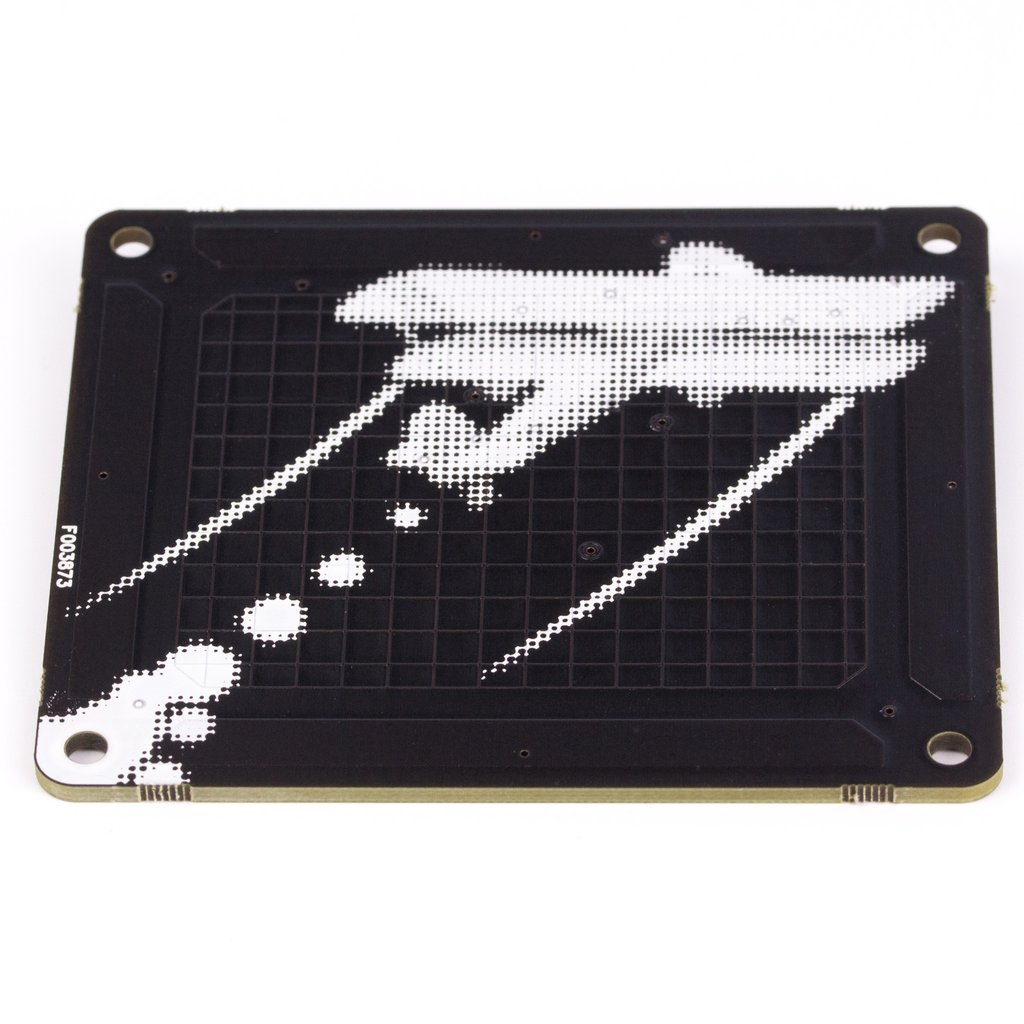
\includegraphics[width=1\textwidth, height=0.6\textheight]{skywriter}
    \caption{Touch Board Skydriver by Piromoni}
    \label{fig:TouchBoard}
\end{figure}

\newpage
%%Bibliografia
\begin{thebibliography}{99}
\raggedright

\bibitem{Raspbian} Raspbian wikipedia, \url{https://it.wikipedia.org/wiki/Raspbian}
\bibitem{Debian} Debian wikidia, \url{https://it.wikipedia.org/wiki/Debian}
\bibitem{Raspberry} Raspberry official website, \url{https://www.raspberrypi.org/}
\bibitem{OpenCV-website} OpenCV official website, \url{http://opencv.org/}
\bibitem{GoogleSTT-website} Google Speech to Text API documentation, \url{https://cloud.google.com/speech/}
\bibitem{Electron-website} Electron official website, \url{https://electron.atom.io/}
\bibitem{MVC-Architecture} MVC Wikipedia, \url{https://en.wikipedia.org/wiki/Model%E2%80%93view%E2%80%93controller}
\bibitem{Express-website} Express official website, \url{http://expressjs.com/it/}
\bibitem{MySQL} MySQL official website, \url{https://www.mysql.com/it/}
\bibitem{Mustache} Mustache Git Site, \url{https://mustache.github.io/}
\bibitem{JavaScript} JavaScript, \url{https://www.javascript.com/}
\bibitem{Python} Python website, \url{https://www.python.it/}
\bibitem{git-website} GitLab website, \url{https://about.gitlab.com/}
\bibitem{NodeJS-website} Nodejs website, \url{https://nodejs.org/it/}
\bibitem{V8} V8 wikipedia, \url{https://it.wikipedia.org/wiki/V8_(motore_JavaScript)}
\bibitem{NPM} npm docs, \url{https://docs.npmjs.com/getting-started/what-is-npm}
\bibitem{Chromium} Chromium wikipedia, \url{https://it.wikipedia.org/wiki/Chromium}
\bibitem{CodeMirror} Chromium wikipedia, \url{https://codemirror.net/}

\end{thebibliography}

\end{document}
